\documentclass[useAMS,usenatbib]{mn2e}
\voffset=-0.1in

%\usepackage{emulateapj5,natbib}
\usepackage{natbib}
\usepackage{amsmath}
\usepackage{url}
\usepackage{longtable}
\usepackage{aas_macros}
\usepackage{amssymb}
\usepackage{graphicx}
\usepackage{deluxetable}

\newcommand{\ugriz}{\protect\hbox{$ugriz$} }
\newcommand{\ugrizyjh}{\protect\hbox{$ugrizY\!\!J\!H$} }
\newcommand{\ugr}{\protect\hbox{$ugr$} }
\newcommand{\gri}{\protect\hbox{$gri$} }
\newcommand{\ri}{\protect\hbox{$ri$} }
\newcommand{\griz}{\protect\hbox{$griz$} }
%\newcommand{\ubvri}{\protect\hbox{$U\!BV\!RI$} }
\newcommand{\ubvrr}{\protect\hbox{$U\!BV\!r$} }
\newcommand{\ubvri}{\protect\hbox{$U\!BV\!ri$} }
\newcommand{\ubv}{\protect\hbox{$U\!BV$} }
\newcommand{\bvri}{\protect\hbox{$BV\!RI$} }
\newcommand{\sbvri}{\protect\hbox{$BV\!ri$} }
\newcommand{\bvrrii}{\protect\hbox{$BV\!rRiI$} }
\newcommand{\ubvgri}{\protect\hbox{$uBV\!gri$} }
\newcommand{\ubvgrrii}{\protect\hbox{$uBV\!grRiI$} }
\newcommand{\bvrijh}{\protect\hbox{$BV\!RI\!J\!H$} }
\newcommand{\ubvrijhk}{\protect\hbox{$U\!BV\!RI\!J\!H\!K$} }
\newcommand{\bvrijhk}{\protect\hbox{$BV\!RI\!J\!H\!K$} }
\newcommand{\vrijhk}{\protect\hbox{$V\!RI\!J\!H\!K$} }
\newcommand{\vri}{\protect\hbox{$V\!RI$} }
\newcommand{\vrizjhk}{\protect\hbox{$V\!RIzJ\!H\!K$} }
\newcommand{\jh}{\protect\hbox{$J\!H$} }
\newcommand{\jhk}{\protect\hbox{$J\!H\!K$} }
\newcommand{\jhks}{\protect\hbox{$J\!H\!K_{s}$} }
\newcommand{\bvz}{\protect\hbox{$BV\!z$} }
\newcommand{\about}{$\sim\!\!$~}
\newcommand{\kms}{\,km\,s$^{-1}$}
\newcommand{\tab}{\hspace*{0.2in}}

\newcommand{\err}[2]{\ensuremath{^{+#1}_{-#2}}}
\newcommand{\msun}{M$_{\sun}$}
\def\lsim{\hbox{\rlap{\raise 0.425ex\hbox{$<$}}\lower 0.65ex\hbox{$\sim$}}}
\def\gsim{\hbox{\rlap{\raise 0.425ex\hbox{$>$}}\lower 0.65ex\hbox{$\sim$}}}
\def\arcmin{\hbox{$^\prime$}}
\def\arcsec{\hbox{$^{\prime\prime}$}}
\def\arcdeg{\mbox{$^\circ$}}

\newcommand{\halpha}{H$\alpha$}
\newcommand{\hbeta}{H$\beta$}
\newcommand{\hgamma}{H$\gamma$}
\newcommand{\hdelta}{H$\delta$}
%\newcommand{\kms}{km~s$^{-1}$ }
\newcommand{\dof}{\rm dof}
\newcommand{\mean}[1]{\left \langle #1 \right \rangle}

\newcommand{\iue}{\protect\hbox{$IU\!E$} }
\newcommand{\hst}{\protect\hbox{$H\!ST$} }
\newcommand{\stis}{\protect\hbox{$ST\!I\!S$} }
\newcommand{\uvot}{\protect\hbox{$UV\!OT$\!\!.} }
\newcommand{\jwst}{\protect\hbox{$JW\!ST$} }

\newcommand{\vsi}{\protect\hbox{$v_{\rm Si\,II}$}}
\newcommand{\vsiz}{\protect\hbox{$v_{\rm Si\,II}^{0}$}}
\newcommand{\vca}{\protect\hbox{$v_{\rm Ca\,H\&K}$}}
\newcommand{\vcaz}{\protect\hbox{$v_{\rm Ca\,H\&K}^{0}$}}

\newcommand\ion[2]{#1$\,${\small{#2}}\relax}


\title[SN~Ia UV CSM]{Searching for Imprints of Circumstellar Material in the Ultraviolet Spectra of Type Ia Supernovae}

\def\illast{1}
\def\illphys{2}

\author[Beaudoin et~al.]{Aaron~Beaudoin$^{\illast,\illphys}$\thanks{E-mail:beaudoi1@illinois.edu},
Ryan~J.~Foley$^{\illast,\illphys}\\
$^{\illast}$Astronomy Department, University of Illinois at Urbana--Champaign, 1002 W.\ Green Street, Urbana, IL 61801, USA\\
$^{\illphys}$Department of Physics, University of Illinois Urbana--Champaign, 1110 W.\ Green Street, Urbana, IL 61801, USA}




\begin{document}

\date{Accepted  . Received   ; in original form  }
\pagerange{\pageref{firstpage}--\pageref{lastpage}} \pubyear{2014}
\maketitle
\label{firstpage}

\begin{abstract}
This is my abstract.
\end{abstract}

\begin{keywords}
  {supernovae: general -- supernovae: individual: SN~2014J}
\end{keywords}


%%%%%%%%%%%%%%%%%%%%
%%  Introduction  %%
%%%%%%%%%%%%%%%%%%%%

\section{Introduction}\label{s:intro}

    Type Ia supernovae (SNe Ia) have relatively homogeneous luminosities, making them excellent probes of dark energy and the expansion of the universe. There are multiple theories regarding their progenitor systems, the first being the single-degenerate (SD) model, which consists of a white dwarf accreting material from either a main-sequence or red-giant star until it reaches the Chandrasekhar mass limit, igniting a thermonuclear explosion. The second model is the double-degenerate (DD) model, which consists of two white dwarfs. However, there is still much uncertainty regarding these systems, and developing a greater understanding of the circumstellar material surrounding SNe Ia is essential in fully understanding these explosions and using them to put greater constraints on dark energy.

    The Na doublet located around 5890 and 5896 angstroms has been measured and analyzed in multiple studies and has shown variability in a handful of cases. This suggests that the Na gas is within 0.5 pc (because of an ionization potential of 5.1 eV) surrounding the SN is ionized by the initial flash. Later, as the Na recombines, absorption features will begin to appear in the SN’s spectrum. However, we need more information from other species with similar ionization potentials to Na in order to determine the circumstellar gas’ location, density, and distribution.

    This work presents the first insight into the Mg II, Mg I, and Fe II absorption features found in the ultraviolet spectrum of 8 SNe Ia, and is the first attempt to probe gas other than Na I, Ca II (not useful because it has a high ionization potential), and K I (not useful because its features are remarkably weak). These features have rest wavelengths of 2796.35 Å and 2803.53 Å for the Mg II doublet, 2852.96 Å for the Mg I line, and 2344.21 Å, 2374.46 Å, 2382.76 Å, 2586.65 Å, and 2600.17 Å for the Fe II lines.

%%%%%%%%%%%%%%%%%%%%
%%  Observations  %%
%%%%%%%%%%%%%%%%%%%%

\section{Observations and Data Reduction}\label{s:obs}

Our sample consists of all SNe~Ia with at least two relatively high resolution ($R > 500$) and high signal-to-noise ratio (S/N) spectra that cover at least the \ion{Mg}{II} doublet.  This limits the sample to 8 SNe~Ia, all observed by the {\it Hubble Space Telescope} ({\it HST}).  With the exception of one SN, all spectra were obtained with the Space Telescope Imaging Spectrograph (STIS).  SN~1992A was observed with the Faint Object Spectrograph (FOS).  Spectra for SNe~1992A, 2011by, 2011fe, 2011iv, and 2014J were first published elsewhere \citep{Kirshner93, Foley12:11iv, Foley14:14j, Foley13:ca, Foley13:met, Mazzali13, Graham14}.  All spectra were reduced in a consistent manner following standard procedures \citep[e.g.,][]{Foley12:11iv}.

Roughly half the sample (X SNe) have only two epochs of spectroscopy, while the other half (X SNe) have $\ge$7 epochs.  Details of the SNe and overall spectroscopic details are presented in Table~\ref{t:sn_info}.  A log of all observations are listed in Table~\ref{t:spec_log}.

In all spectra, we see clear narrow absorption features from the \ion{Mg}{II} doublet.  However, for three SNe, only lines consistent with Milky Way absporption are detected (SNe~1992A, 2011iv, and 2011ek).  This is not unexpected for these objects since SNe~1992A and 2011iv have early-type hosts and SN~2011ek occurs at a projected distance of $>$10~kpc from its host.  For the other 5 SNe~Ia, we detect mesurable \ion{Mg}{II} in at least one spectrum.  For all SNe with detectable \ion{Mg}{II}, we have also detected \ion{Mg}{I} $\lambda$2851.  Only SN~2011fe has detectable \ion{Fe}{II} absorption. {\bf Update this}

%%%%%%%%%%%%%%%%
%%  Analysis  %%
%%%%%%%%%%%%%%%%

\section{Analysis}\label{s:anal}

With detections of several absorption features, we now detail how we make our EW measurements, determine limits for undetected lines, and verify our measurements.

In order to measure the EWs of the narrow absorption features, we first fit either a 3rd order b-spline or a 5th order b-spline to the continuum, based on the S/N of the spectrum.  Dividing by this function, we generate a normalized spectrum.  Because the spectral resolution is low enough where the absorption features are unresolved, we fit Gaussian functions to the absorption features using a least-squares minimization.  Because of the low S/N of some spectra this method is preferable to a direct measurement, which can be significantly biased by the exact wavelength range chosen for integration. Then, we integrate over this Gaussian function to measure the equivalent width of each absorption feature, and use Equation~\ref{e:err} to determine the statistical error.
\begin{equation}
  \sigma_{\rm tot}^{2} = \sqrt{\pi} \times (\sigma_{h}^{2} \times w^{2} + \sigma_{w}^{2} \times h^{2}),
\end{equation}\label{e:err}
where $w$ and $h$ are the width and height of the feature.

For SNe~2011by, 2012cg, and 2013dy, the Milky Way \ion{Mg}{II} $\lambda$2803 line overlaps in wavelength with the host-galaxy \ion{Mg}{II} $\lambda$2796 line.  {\bf For 11fe, both lines overlap.}  For these objects, we fit the entire feature (both \ion{Mg}{II} doublets) with two \ion{Mg}{II} doublets, one at zero velocity and the other at roughly the recession velocity of the host galaxy, simultaneously.  Because of degeneracies in the fitting, we fixed each line from a given doublet to have the same shape.  As a result for these objects, the EW for one \ion{Mg}{II} line is equivalent to that of the other.  However, the additional data from the the overlapping line is useful for constraining parameters and improves the accuracy of the EW measurement.

In addition to the statistical uncertainties determined during the Gaussian fitting, we estimated the systematic uncertainites, mostly resulting from uncertain continuum placement, through a Monte Carlo simulation.  For each realization of the Monte Carlo simulation, we shift the nominal wavelength of the b-spline breakpoints and redetermine the continuum.  The amplitude of the shifts were chosen such that the continuum was not obviously incorrect for 500 sample trials.  We then remeasure the EWs of each line with the new normalized spectrum.  The scatter in the resulting distribution of EW measurements was used to determine the systematic uncertainty.  The statistical and systematic uncertainties were combined for our total uncertainty.

For SN~1992A, 2011ek, and 2011iv, we determined the magnitude necessary for each absorption feature to be able to be resolved in the noise of a specific normalized spectrum. {\bf But you need to do this for all spectra with any non-detections, not just these three SNe; and re-write this to state first that we are trying to determine the detection limit and then talk about what you do to get there.}  This 3-$\sigma$ limit is determined with Equation~\ref{e:limit}, taken from \citep{Leonard01},
\begin{equation}
W_{\lambda}(3\sigma) = 3 \Delta \lambda \Delta I \sqrt{\frac{W_{\rm line}}{\Delta \lambda}} \sqrt{\frac{1}{B}},
\end{equation}\label{e:limit}
where $W_{\rm line}$ is the estimated width of the feature, $\Delta \lambda$ is roughly 2 pixels or 3 $\AA$, $\Delta I$ is the RMS of the spectrum in that specific area, and $B = 2$ (the number of bins per resolution element). {\bf Fix this up; I think a bunch of these variables need to be defined differently.}

\section{Results}\label{s:results}

\begin{figure}
\begin{center}
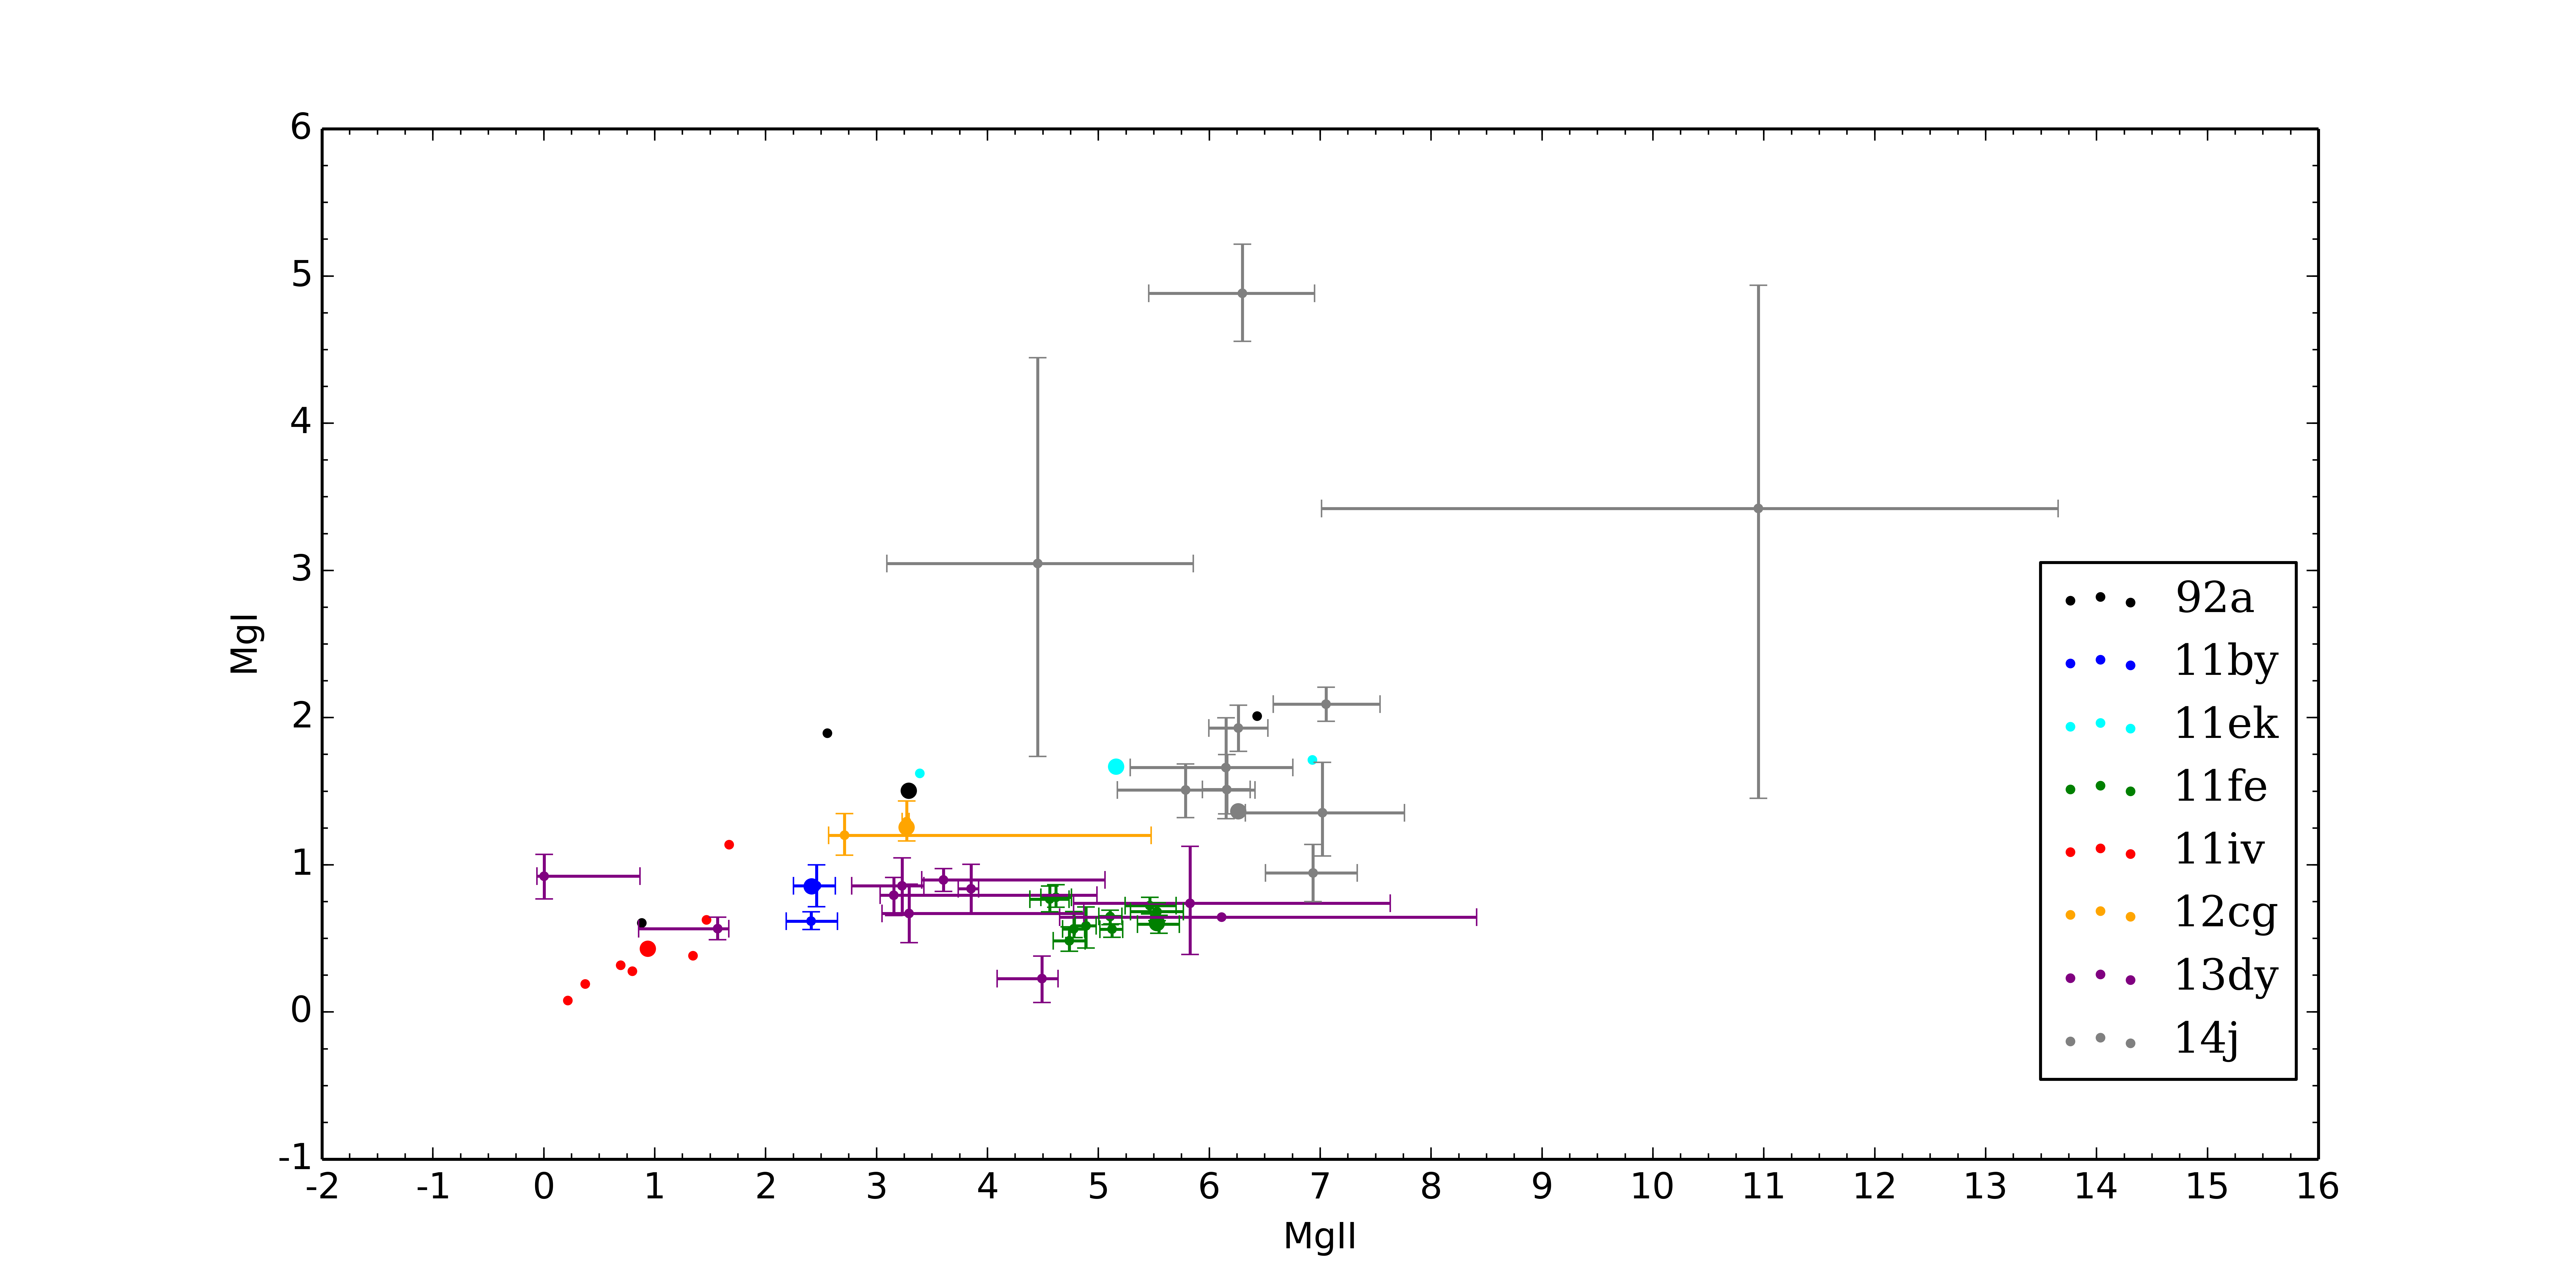
\includegraphics[angle=0,width=3.2in]{mgi_vs_mgii}
\caption{Update caption.}\label{f:lc}
\end{center}
\end{figure}

\section{Discussion}\label{s:disc}

\section{Future Work}\label{s:fw}

\begin{deluxetable}{llllllllll}
\tabletypesize{\footnotesize}
\tablewidth{0pt}
\tablecaption{Measurements of Observed SNe \label{t:sne}}
\tablehead{
\colhead{UT} & \colhead{Phase} & \colhead{\ion{Fe}{II}} & \colhead{FeII} & \colhead{FeII)} & \colhead{FeII} & \colhead{FeII} & \colhead{MgII} & \colhead{MgII} & \colhead{MgI}\\
\colhead{(days)} & \colhead{(d)} & \colhead{(2344.22 \AA)} & \colhead{(2374.46 \AA)} & \colhead{(2382.76 \AA)} & \colhead{(2586.65 \AA)} & \colhead{(2600.17 \AA)} & \colhead{(2796.35 \AA)} & \colhead{(2803.53 \AA)} & \colhead{(2852.96 \AA)}
}

\startdata
\multicolumn{10}{c}{SN~1992A}\\
$19920124.21$ & $4.98$ & $0.91$ & $1.44$ & $1.59$ & $1.59$ & $1.84$ & $0.32$ & $0.57$ & $0.6$\\
$19920304.31$ & $44.83$ & $1.81$ & $1.78$ & $3.06$ & $5.03$ & $4.75$ & $1.3$ & $1.25$ & $1.89$\\
$19921105.59$ & $289.58$ & $138.94$ & $14.32$ & $52.77$ & $95.3$ & $95.35$ & $3.37$ & $3.06$ & $2.01$\\
\multicolumn{10}{c}{SN~2011by}\\
$20110430.56$ & $-9.31$ & $1.24$ & $1.33$ & $1.34$ & $0.8$ & $0.54$ & $1.23^{+0.12}_{-0.15}$ & $1.23^{+0.12}_{-0.15}$ & $0.86^{+0.14}_{-0.14}$\\
$20110509.38$ & $-0.52$ & $0.59^{+0.1}_{-0.13}$ & $1.25^{+0.32}_{-0.3}$ & $1.12^{+0.17}_{-0.17}$ & $1.15^{+0.29}_{-0.29}$ & $0.78^{+0.04}_{-0.04}$ & $1.21^{+0.18}_{-0.16}$ & $1.2^{+0.16}_{-0.16}$ & $0.62^{+0.06}_{-0.06}$\\
\multicolumn{10}{c}{SN~2011ek}\\
$20110812.56$ & $-3.32$ & $4.27$ & $6.44$ & $5.52$ & $4.32$ & $6.2$ & $2.01$ & $1.38$ & $1.62$\\
$20110819.45$ & $3.53$ & $6.54$ & $14.03$ & $51.01$ & $70.52$ & $93.52$ & $3.56$ & $3.37$ & $1.71$\\
\multicolumn{10}{c}{SN~2011fe}\\
$20110828.17$ & $-13.11$ & $2.17^{+0.41}_{-0.57}$ & $1.24^{+0.05}_{-0.07}$ & $3.45^{+0.3}_{-0.34}$ & $1.66^{+0.66}_{-0.71}$ & $2.33^{+0.65}_{-1.01}$ & $2.56^{+0.12}_{-0.12}$ & $2.0^{+0.13}_{-0.14}$ & $0.77^{+0.09}_{-0.09}$\\
$20110831.27$ & $-10.04$ & $1.37^{+0.51}_{-0.21}$ & $1.05^{+0.09}_{-0.09}$ & $2.0^{+0.19}_{-0.19}$ & $2.28^{+0.24}_{-0.4}$ & $2.0^{+0.16}_{-0.28}$ & $2.44^{+0.12}_{-0.12}$ & $2.29^{+0.07}_{-0.07}$ & $0.48^{+0.09}_{-0.07}$\\
$20110903.43$ & $-6.91$ & $1.36^{+0.06}_{-0.06}$ & $0.95^{+0.1}_{-0.1}$ & $1.9^{+0.11}_{-0.11}$ & $1.3^{+0.21}_{-0.17}$ & $1.83^{+0.19}_{-0.18}$ & $2.92^{+0.14}_{-0.14}$ & $2.55^{+0.19}_{-0.17}$ & $0.72^{+0.06}_{-0.06}$\\
$20110907.42$ & $-2.95$ & $1.5^{+0.08}_{-0.08}$ & $0.75^{+0.02}_{-0.02}$ & $1.92^{+0.05}_{-0.05}$ & $1.17^{+0.2}_{-0.18}$ & $1.91^{+0.09}_{-0.06}$ & $2.92^{+0.1}_{-0.1}$ & $2.61^{+0.21}_{-0.21}$ & $0.68^{+0.06}_{-0.06}$\\
$20110910.44$ & $0.04$ & $1.21^{+0.05}_{-0.05}$ & $0.85^{+0.05}_{-0.04}$ & $1.93^{+0.07}_{-0.07}$ & $1.06^{+0.17}_{-0.16}$ & $1.75^{+0.09}_{-0.08}$ & $2.88^{+0.1}_{-0.12}$ & $2.66^{+0.16}_{-0.16}$ & $0.6^{+0.06}_{-0.06}$\\
$20110913.68$ & $3.25$ & $2.51^{+0.36}_{-0.37}$ & $1.09^{+0.29}_{-0.26}$ & $1.59^{+0.25}_{-0.23}$ & $1.28^{+0.4}_{-0.38}$ & $1.73^{+0.27}_{-0.26}$ & $2.96^{+0.04}_{-0.03}$ & $2.15^{+0.1}_{-0.1}$ & $0.65^{+0.04}_{-0.06}$\\
$20110919.63$ & $9.15$ & $1.44^{+0.1}_{-0.1}$ & $0.71^{+0.0}_{-0.01}$ & $1.78^{+0.1}_{-0.1}$ & $1.17^{+0.04}_{-0.05}$ & $1.77^{+0.05}_{-0.07}$ & $2.7^{+0.04}_{-0.08}$ & $2.43^{+0.09}_{-0.08}$ & $0.56^{+0.04}_{-0.05}$\\
$20111001.27$ & $20.69$ & $1.66^{+0.1}_{-0.11}$ & $0.69^{+0.13}_{-0.13}$ & $1.64^{+0.22}_{-0.12}$ & $1.16^{+0.18}_{-0.32}$ & $1.77^{+0.31}_{-0.52}$ & $2.59^{+0.09}_{-0.09}$ & $2.19^{+0.03}_{-0.04}$ & $0.56^{+0.12}_{-0.06}$\\
$20111007.32$ & $26.69$ & $1.21^{+0.09}_{-0.09}$ & $1.25^{+0.09}_{-0.11}$ & $1.88^{+0.14}_{-0.18}$ & $0.89^{+0.18}_{-0.15}$ & $1.52^{+0.43}_{-0.35}$ & $2.68^{+0.05}_{-0.05}$ & $2.21^{+0.08}_{-0.08}$ & $0.59^{+0.13}_{-0.15}$\\
$20111021.2$ & $40.45$ & $1.31^{+0.15}_{-0.15}$ & $0.93^{+0.12}_{-0.12}$ & $1.93^{+0.16}_{-0.17}$ & $0.95^{+0.11}_{-0.1}$ & $2.19^{+0.18}_{-0.18}$ & $2.78^{+0.1}_{-0.11}$ & $1.84^{+0.09}_{-0.08}$ & $0.78^{+0.09}_{-0.07}$\\
\multicolumn{10}{c}{SN~2011iv}\\
$20111211.1$ & $0.6$ & $0.22$ & $0.15$ & $0.12$ & $0.15$ & $0.17$ & $0.09$ & $0.13$ & $0.08$\\
$20111215.94$ & $5.41$ & $0.45$ & $0.42$ & $0.43$ & $0.39$ & $0.27$ & $0.18$ & $0.19$ & $0.19$\\
$20111220.72$ & $10.15$ & $0.71$ & $0.45$ & $0.62$ & $0.36$ & $0.45$ & $0.3$ & $0.39$ & $0.32$\\
$20111224.58$ & $13.99$ & $1.24$ & $0.89$ & $1.13$ & $0.5$ & $0.55$ & $0.46$ & $0.34$ & $0.28$\\
$20111228.44$ & $17.82$ & $0.78$ & $1.55$ & $1.47$ & $0.78$ & $0.68$ & $0.66$ & $0.69$ & $0.38$\\
$20120101.36$ & $21.72$ & $1.01$ & $1.28$ & $1.1$ & $0.67$ & $0.81$ & $0.55$ & $0.92$ & $0.63$\\
$20120109.21$ & $29.52$ & $1.03$ & $1.0$ & $1.28$ & $1.03$ & $1.13$ & $0.95$ & $0.72$ & $1.14$\\
\multicolumn{10}{c}{SN~2012cg}\\
$20120604.5$ & $2.5$ & $1.86$ & $1.59$ & $1.43$ & $0.86$ & $0.51$ & $1.36^{+2.24}_{-0.1}$ & $1.35^{+1.62}_{-0.1}$ & $1.2^{+0.15}_{-0.14}$\\
$20120618.4$ & $16.37$ & $2.96$ & $1.6$ & $1.35$ & $1.09$ & $1.46$ & $1.64^{+0.02}_{-0.03}$ & $1.63^{+0.02}_{-0.03}$ & $1.29^{+0.14}_{-0.13}$\\
\multicolumn{10}{c}{SN~2013dy}\\
$20130721.5$ & $-6.17$ & $3.07^{+0.52}_{-0.59}$ & $1.37^{+0.11}_{-0.17}$ & $0.86^{+0.29}_{-0.32}$ & $3.86^{+0.29}_{-0.29}$ & $2.4^{+1.69}_{-1.69}$ & $1.58^{+1.32}_{-0.09}$ & $1.58^{+1.27}_{-0.08}$ & $0.79^{+0.12}_{-0.14}$\\
$20130725.61$ & $-2.09$ & $0.86$ & $1.37$ & $1.33$ & $2.78^{+0.43}_{-0.43}$ & $1.63^{+0.28}_{-0.28}$ & $0.0^{+0.81}_{-0.06}$ & $0.0^{+0.3}_{-0.02}$ & $0.92^{+0.15}_{-0.15}$\\
$20130727.34$ & $-0.37$ & $0.59$ & $1.76$ & $1.36$ & $2.31^{+0.73}_{-0.99}$ & $1.01^{+0.95}_{-0.61}$ & $1.62^{+0.14}_{-0.33}$ & $1.61^{+0.14}_{-0.31}$ & $0.86^{+0.19}_{-0.2}$\\
$20130729.32$ & $1.61$ & $0.91$ & $1.19$ & $1.03$ & $2.63^{+0.61}_{-0.61}$ & $1.0^{+0.58}_{-0.35}$ & $1.65^{+1.19}_{-0.17}$ & $1.64^{+1.03}_{-0.17}$ & $0.67^{+0.2}_{-0.2}$\\
$20130801.59$ & $4.85$ & $1.21$ & $0.86$ & $0.92$ & $2.31^{+0.33}_{-0.33}$ & $0.82^{+0.49}_{-0.49}$ & $0.85^{+0.08}_{-0.48}$ & $0.72^{+0.06}_{-0.53}$ & $0.57^{+0.08}_{-0.07}$\\
$20130805.51$ & $8.76$ & $1.63^{+0.41}_{-0.36}$ & $1.89^{+0.74}_{-0.79}$ & $1.33^{+1.01}_{-0.68}$ & $2.09^{+0.45}_{-0.46}$ & $1.77^{+0.76}_{-1.02}$ & $1.81^{+1.1}_{-0.14}$ & $1.8^{+0.96}_{-0.14}$ & $0.9^{+0.08}_{-0.08}$\\
$20130809.11$ & $12.36$ & $1.22$ & $1.66$ & $0.76$ & $3.53^{+1.11}_{-1.33}$ & $3.24^{+0.79}_{-1.31}$ & $1.93^{+0.05}_{-0.08}$ & $1.92^{+0.05}_{-0.08}$ & $0.84^{+0.17}_{-0.17}$\\
$20130811.15$ & $14.38$ & $3.22^{+1.0}_{-1.05}$ & $2.86^{+0.78}_{-0.99}$ & $3.68^{+1.51}_{-1.75}$ & $1.15$ & $1.16$ & $2.26^{+0.11}_{-0.28}$ & $2.23^{+0.1}_{-0.29}$ & $0.23^{+0.15}_{-0.16}$\\
$20130815.01$ & $18.22$ & $2.02$ & $1.62$ & $1.32$ & $0.95$ & $2.35$ & $3.29^{+1.78}_{-1.07}$ & $2.82^{+1.46}_{-0.99}$ & $0.64$\\
$20130817.94$ & $21.17$ & $1.98$ & $1.63$ & $1.68$ & $2.64^{+0.24}_{-0.24}$ & $1.57^{+0.55}_{-1.12}$ & $2.82^{+1.29}_{-0.73}$ & $3.01^{+1.26}_{-0.75}$ & $0.74^{+0.39}_{-0.35}$\\
\multicolumn{10}{c}{SN~2014J}\\
$20140126.6$ & $-6.5$ & $19.25$ & $12.14$ & $22.8$ & $3.36$ & $2.36$ & $2.97^{+0.17}_{-0.17}$ & $3.18^{+0.13}_{-0.13}$ & $1.51^{+0.24}_{-0.16}$\\
$20140128.44$ & $-4.5$ & $10.63$ & $6.34$ & $5.55$ & $2.62$ & $1.84$ & $3.05^{+0.19}_{-0.19}$ & $3.21^{+0.18}_{-0.18}$ & $1.93^{+0.16}_{-0.16}$\\
$20140130.49$ & $-2.5$ & $19.39$ & $34.54$ & $37.38$ & $2.64$ & $3.69$ & $3.62^{+0.32}_{-0.29}$ & $3.43^{+0.37}_{-0.38}$ & $2.09^{+0.12}_{-0.12}$\\
$20140201.61$ & $-0.5$ & $33.05$ & $21.6$ & $56.35$ & $4.7$ & $2.27$ & $3.52^{+0.41}_{-0.43}$ & $3.5^{+0.61}_{-0.55}$ & $1.35^{+0.34}_{-0.29}$\\
$20140204.73$ & $2.5$ & $36.54$ & $167.71$ & $79.96$ & $5.04$ & $7.22$ & $3.3^{+0.49}_{-0.77}$ & $2.85^{+0.35}_{-0.4}$ & $1.66^{+0.34}_{-0.35}$\\
$20140208.53$ & $6.5$ & $32.87$ & $17.37$ & $17.95$ & $4.88$ & $2.88$ & $2.72^{+0.4}_{-0.42}$ & $3.07^{+0.48}_{-0.45}$ & $1.51^{+0.18}_{-0.19}$\\
$20140210.44$ & $8.49$ & $184.37$ & $9.1$ & $16.32$ & $4.25$ & $4.25$ & $3.28^{+0.21}_{-0.25}$ & $3.66^{+0.34}_{-0.35}$ & $0.94^{+0.19}_{-0.19}$\\
$20140213.29$ & $11.49$ & $8.08$ & $35.36$ & $10.33$ & $172.19$ & $168.98$ & $3.5^{+0.36}_{-0.42}$ & $2.8^{+0.54}_{-0.73}$ & $4.88^{+0.33}_{-0.33}$\\
$20140216.41$ & $14.49$ & $16.24$ & $9.44$ & $217.64$ & $5.09$ & $7.04$ & $2.47^{+1.17}_{-1.1}$ & $1.98^{+0.78}_{-0.8}$ & $3.05^{+1.4}_{-1.31}$\\
$20140226.07$ & $24.05$ & $11.52$ & $23.68$ & $6.04$ & $17.56$ & $106.42$ & $5.6^{+1.79}_{-3.05}$ & $5.35^{+2.03}_{-2.49}$ & $3.42^{+1.52}_{-1.97}$\\

\enddata


\end{deluxetable}


\bibliographystyle{mn2e}
\bibliography{astro_refs}

\label{lastpage}

%\eject

\end{document}